\chapter{Improved Viola-Jones Object Detection for Landmark Extraction}
\label{chap:five}

Viola-Jones object detection algorithm \cite{violajones} is a gold-standard in computer vision to detect trained objects at a very high speed using boosted classifiers. Because of their speed, they are used for object detection based landmark extraction in SLAM. In our multi-robot evaluation dataset, all the robots are fitted with a unique fiducial to represent their identity. Apart from this, the environment also contains fiducial markers that can be considered as landmarks in the map. In order to detect these with at a much lower false positive rate, at a lower resolution and eventually at a higher speed we improve the algorithm to utilize all the color channels in the input image. The original version works only on grayscale images. The key requirements for our scenario include high detection percentage with lower false positive rate and more importantly, the detection of the fiducial markers at various scale. As the robots are navigating, the target fiducial may come near or move away resulting in change in the size of fiducial on the captured image over continuous frames. The Haar features in Viola-Jones algorithm are perfectly suitable for this as they are scale invariant. We retain this property of the algorithm and increase the detection percentage along with the detection speed by leveraging the additional information obtained by using all the channels of the image. The improved version uses the same metric used in the original version to score a Haar feature but does it for all the channels of the input image. Thus the score is represented as a vector as opposed to a scalar value in the original version. These vectors are then ranked using linear discriminant analysis. We train a classifier to detect these fiducial markers using this improved version of Viola-Jones algorithm. The increase in the time complexity is matched by the ability to achieve better detection rates at lower resolution thereby producing a lower detection time overall. 
\paragraph{}
Since the detection algorithm and in general SLAM problem is very time sensitive, it is important to understand how the various tunable parameters affect the detection time. This chapter focuses on the complexity analysis of the multi-scale and multi-channel decision tree based detector. The algorithm learns a decision tree during the training stage which is usually evaluated on the test image set using a sliding window approach for multiple sizes of the window (scale invariance). In the next section, I would shed some light on few relevant works that have extended the original work of Viola-Jones in different contexts such as improving false alarm rate, modifications in Haar features, weighting schemes in Adaboost etc. There is no particular work that specifically deals with a detailed theoretical complexity analysis of the final detector although there has been empirical analysis both in the original paper \cite{violajones} and \cite{classifier4}. These theoretical results would be followed by a few experiments in the final section.

\section{Related Work}
In Viola-Jones object detection algorithm \cite{violajones}, the integral image for feature computation, Adaboost for feature selection and an attentional cascade for efficient computational resource allocation are the three key components behind achieving very high processing speed although the performance is same as the previous complex single stage classifiers. Following that, Lienhart \textit{et. al,} \cite{classifier4} did an empirical analysis of the original work and also introduced $45^{o}$ rotated HAAR features and verified that the Gentle Adaboost performs better than Real and Discrete Adaboost in terms of detection accuracy. A complete algorithmic description that explains the implementation logic behind Open Computer Vision library \cite{classifier14} is provided by \cite{classifier13}. Almost all the previously existing analysis deal only with the complexity of training the Cascade Classifier and just mention that the detection rate is very fast. To the best of my knowledge, this is the first analysis of the computational complexity of the Cascade Classifier object detection as a function of various tunable parameters.

\section{Theoretical Results}
The trained classifier performs a sliding window search over the target image for a fixed window size during every iteration. The set of tunable parameters for the Cascade Classifier Detector are:

\begin{itemize}
    \item The minimum window width and height of search, $W_{min}$ = $\{ w_{min}$, $h_{min} \}$
    \item The maximum window width and height of search, $W_{max}$ = $\{ w_{max}$, $h_{max} \}$
    \item The scale factor by which the window size grows from minimum to maximum, $\gamma_0$
    \item The minimum number of detections in the neighborhood to be selected as a true positive, $\beta$
\end{itemize}

\paragraph{}
The classifier is a cascaded set of decision trees and the number of such decision trees and the depth of each tree also influences the total time. However, since this value is constant for a given classifier it cannot be considered as a part of tunable parameters. Nevertheless, I have mentioned an upper bound on the number of evaluations of the entire decision tree over a given image. \\
\textbf{REMARK:} The classifier cannot detect target objects smaller than the trained window size. 

\subsection{Search window size and scale factor}
The maximum and minimum window sizes and the scale factor are interrelated and hence considered together for analysis. The size of the window along both the width and height is increased from the minimum to maximum value at the scale factor ratio. This is done to stick to the constant aspect ratio at which the classifier is trained. Let $w_t$ and $h_t$ be the training width and height. The set of all scale factor values is given by

\begin{equation}
\Gamma = \{ \gamma \mid w_t.\gamma \in [w_{min}, w_{max}] \cap h_t.\gamma \in [h_{min}, h_{max}], \gamma = \gamma_0, \gamma_0^2, ... ,\gamma_0^n\} \  \forall \ n \in \mathbb{N}     
\label{eq1}
\end{equation} 

%todo change "finer search window size."
where $\gamma_0$ is the initial value of scale factor which is also equal to the one input by the user. Generally, it is advised that $\gamma_0$ be in the positive neighborhood of 1, $\gamma_0 \rightarrow 1_+$ to get a finer search window size. The set of scale factors form a geometric progression with $\gamma_0$ being the common ratio between subsequent values. Now the set of image resolutions for which the integral image is to be calculated is given by 

\begin{equation}
I = \{ (x, y) | x = \frac{w_t}{r}, y = \frac{h_t}{r}\} \ \forall \ r \in \Gamma
\label{eq2}
\end{equation} 


\paragraph{}
The integral image is calculated for $\mid I \mid$ number of times. The number of elements in the set $I$ is actually the number of terms in the G.P represented by $\Gamma$ which can be calculated as follows.

\paragraph{}
Let $i$ denote the index of the terms in a G.P formed by initial value 1 and common ratio $\gamma_0$. Then the least and greatest value of $i$ that scales $w_t$ to the range $[w_{min}, w_{max}]$ are 

\begin{equation}
i^w_l = \left \lceil log_{\gamma_0} \left ( \frac{w_{min}}{w_t} \right ) \right \rceil
\label{eq3}
\end{equation}

\begin{equation}
i^w_g = \left \lfloor log_{\gamma_0} \left ( \frac{w_{max}}{w_t} \right ) \right \rfloor
\label{eq4}
\end{equation}

where the subscripts $l$ and $g$ represent the least and greatest index values respectively and $\lfloor.\rfloor$ and $\lceil.\rceil$ are the least and greatest integer functions.

\paragraph{}
Similarly, the least and greatest value of $i$ that scales $h_t$ to the range $[h_{min}, h_{max}]$ are 

\begin{equation}
i^h_l = \left \lceil log_{\gamma_0} \left ( \frac{h_{min}}{h_t} \right ) \right \rceil
\label{eq5}
\end{equation}

\begin{equation}
i^h_g = \left \lfloor log_{\gamma_0} \left ( \frac{h_{max}}{h_t} \right ) \right \rfloor
\label{eq6}
\end{equation}


\paragraph{}
To stick with the aspect ratio, only the terms that are common between the set of width and set of height ratios are considered. The number of common scale factors $K$ which is same as  $\mid \Gamma \mid$ and $\mid I \mid$ is in turn given by

\begin{equation}
K = \mid \Gamma \mid = \mid I \mid = min \{ i_g^w - i_l^w, i_g^h - i_l^h \}
\label{eq7}
\end{equation}

\begin{equation}
K = min \left \{ \left \lceil log_{\gamma_0} \left ( \frac{w_{max}}{w_{min}} \right ) \right \rceil , \left \lceil log_{\gamma_0} \left ( \frac{h_{max}}{h_{min}} \right ) \right \rceil \right \}
\label{eq8}
\end{equation}

Using the change of base rule,

\begin{equation}
K = min \left \{ \left \lceil \frac{ln \left ( \frac{w_{max}}{w_{min}} \right )}{ln\  \gamma_0}  \right \rceil , \left \lceil \frac{ln \left ( \frac{h_{max}}{h_{min}} \right )}{ln \ \gamma_0}  \right \rceil \right \}
\label{eq9}
\end{equation}


\paragraph{}
All example sub-windows used for training were variance normalized to minimize the effect of different lighting conditions. Normalization is therefore necessary during
detection as well. The variance of an image sub-window can be computed quickly using a pair of integral images. Recall that $\sigma^2 = m^2 - \frac{1}{N}\sum x^2$, where $\sigma$ is the standard deviation, $m$ is the mean, and $x$ is the pixel value within the sub-window. The mean of a sub-window can be computed using the integral image. The sum of squared pixels is computed using an integral image of the image squared (i.e. two integral images are used in the scanning process). During detection the effect of image normalization can be achieved by post-multiplying the feature values rather than pre-multiplying the pixels. Thus the integral image is calculated $2K$ number of times. The integral image is a summed area table data structure which is calculated  efficiently using a recursive algorithm. Though the computation of summed area table depends on the resolution of the image, the task of evaluating the intensities over any rectangular area requires only four array references. This allows for a constant calculation time that is independent of the size of the rectangular area. Also for multichannel images with $M$ channels, the number of integral image computations is $2MK$ times. This factor $M$ is the \textit{only} significant difference between multichannel cascade classifier detector and grayscale detector.

\subsection{Minimum number of neighbors}

The element set containing multiple detections of differently sized objects in target images are split into equivalency classes (clustering). We use a first order logic with a predicate that relates the objects in the set based on the test of similarity of rectangles. The running time of the clustering algorithm is actually \textit{independent} of the threshold $\beta$ that corresponds to the minimum number of neighbors jointly satisfying the predicate. The logic implements an $\mathcal{O}(N^2)$ algorithm for clustering a set of $N$ elements into one or more equivalency classes \cite{classifier1} as described using disjoint-set data structure representation \cite{classifier2}. For every element in the disjoint-set data structure of size $N^2$ the predicate is evaluated which returns either true or false. 
\paragraph{}
The predicate evaluates similarity of rectangles by taking any two elements from the input set along with the internal parameter $\epsilon$, $0 < \epsilon < 1$. \\

\setlength\parindent{24pt}
\textit{\textbf{Lemma:}}\textit{Two rectangles are similar if their sides are proportional.} 

\paragraph{}
This is checked by finding if all the sides of one rectangle is within $\Delta$ $=$ $\epsilon * (min(w_1, w_2),$ $min(h_1, h_2)) / 2$ of the other rectangle. \\
%todo formulate the necessity of a metric and why you need it. Then introduce delta

\setlength\parindent{24pt}
\textit{\textbf{Lemma:}}\textit{Two rectangles which are within a threshold $\Delta$ on all the four sides, for a $\Delta$ formulated using \textit{minimum} of width and height of the participating rectangles, are also within a threshold $\Delta$ for a $\Delta$ formulated using the maximum of their width and height.} 

\paragraph{}
Hence a $\Delta$ formed by the minimum of the their sides is a more restricted metric. The reason for formulating $\Delta$ is to account of uncertainty in similarity. The representative rectangle for all the equivalency class in the disjoint-set data structure is obtained by averaging all the constituent rectangles which is in turn returned as the detected rectangle. 

\subsection{Depth of the decision tree and target image resolution}

Though it looks like the detector is evaluated for various window sizes from minimum to maximum size, algorithmically the target image is shrunk from its original resolution to various sizes depending upon scale factors such that the objects of interest of sizes between minimum and maximum window size falls inside the constant window size. In other words, we are decreasing the size of the target image itself rather than increasing the size of the search window and rescaling the features appropriately. We take this rather long route of rescaling the image because the detection could be done using the same window size by which the classifier is trained. Although the values of the feature learned at every level of the classifier is normalized by the area of the feature, no clear explanation about guarantees on generality of learned classifier value for arbitrary rescaling of the feature considering linear interpolation of image and truncation/round-off errors in feature rescaling is given in the original paper \cite{violajones}. Obviously, by fractional rescaling the new correct positions become fractional. A plain vanilla solution is to round all relative look-up positions to the nearest integer position. However, performance may degrade significantly, since the ratio between the two areas of a feature may have changed significantly compared to the area ratio at training due to rounding. One solution is to correct the weights of the different rectangle sums so that the original area ratio between them for a given haar-like feature is the same as it was at the original size \cite{classifier4}. Nevertheless, by doing this reverse operation we end up linearly decimating the target image $\mid \Gamma \mid$ times and calculating integral image for each of them. From a memory perspective, the integral image for all the scales of the target image are computed and stored in a continuous serial buffer of size

$$ M \times \sum_{\gamma \in \Gamma} \left ( \frac{W}{\gamma} + 1 \right ) \left ( \frac{H}{\gamma} + 1  \right ) $$

where $W \times H$ is the resolution, $M$ is the number of channels of the target image and $\Gamma$ is the set of scale factors.

\paragraph{}
For a decision tree of $S$ stages and depth $d_s$ per stage where $s \in S$, an upper bound on the number of evaluations of all the stages of the decision tree is given by 

\begin{equation}
\le \sum_{\gamma \in \Gamma} \left \{ \left ( \frac{W}{\gamma} - w_t + 1 \right ) \left ( \frac{H}{\gamma} - h_t + 1  \right ) \times \sum_{s \in S} d_s \right \}
\label{eq10}
\end{equation}

where $W \times H$ is the resolution of the target image, $w_t \times h_t$ is the training resolution and $\Gamma$ is the set of all scale factors. 
\paragraph{}
\textbf{Note}: An implementation detail is that, for integral image resolutions whose corresponding scale factor is less than 2, the cascaded decision tree is only evaluated over every other pixel along width and height. Also, the entire continuous buffer of integral image across various resolutions is striped into memory chunks of size 

\begin{equation}
\delta_i = 32 \times \frac{H}{\gamma_i W} \  \ \forall \gamma_i \in \Gamma
\label{eq11}
\end{equation}


where $32$ is code specific. In total, there are $\sum_i \delta_i$ chunks which are processed in parallel using TBB multi-threading library.


\section{Experiments run}
% {\it Note: Describe in as much detail as possible the experiments that you
% set up and ran over this week. These could have been exploratory ones to
% understand an algorithm/tool/package/domain/dataset/programming model, etc.
% These could have been proof of concept experiments run on synthetic data or
% small samples. The experiments could have succeeded or failed. But for each
% of the experiments, you should write down clearly why you decided to run the
% experiment. What was the set up? All the parameters used, no. of runs, etc.
% Document all the outcomes clearly. Which parameter settings did the
% experiment succeed, when did it fail. Why did you choose a certain setting?
% Tabulate things clearly.. and where possible, draw graphs/charts etc.

% Clearly document your code as well. Keep around different versions, with
% comments describing what is different in each version. Try to follow some
% coding standards. In experiments that take a long time to run, save as much
% of the intermediate computation as possible. Do not write out only averages
% to the file. This might take slightly longer to run initially, but will save
% a lot of time when needing to re-run the experiments. For example, if you
% want to do some feature computation and then run a classifier on some data,
% save the computed features also. That way when you want to run a new
% classifier you don't have to compute features again.}
%"change ref in  span of a typically setup storeaisle shelf as shown in Fig.\ref"
The Haar Cascade Classifier \cite{violajones} described so far is used to detect the fiducial markers on top of every robot and in the environment in an online fashion. The biggest advantage of the Cascade Classifiers are their rapid speed of detection despite very long training time. The complexity analysis summarised in this report gives an idea on the sensitivity of each classifier parameter on the detection time. A conservative search size may detect all object instances but it is time critical to have a tight estimate that is just enough to detect all such instances.
\paragraph{}
From the theoretical results, it is clear how different values of the parameters are mathematically related. For this experiment we trained a fiducial marker with a training window size $63 \times 35$ using Gentle Adaboost \cite{classifier6,classifier7}.  In order to prove that the detection time is logarithmically related to the size of the search space defined by maximum and minimum window size, I ran the algorithm with multiple search search sizes decided by minimum and maximum window size. For the simplicity of understanding and denoting, the search size $\mathcal{S}$ can be represented as the length of line joining the right bottom corners of the minimum and maximum sized search rectangles.
\begin{equation}
\mathcal{S} = \sqrt{w_{max}^2 + h_{max}^2} - \sqrt{w_{min}^2 + h_{min}^2}
\label{eq12}
\end{equation}

\begin{figure}[h]
    \centering
    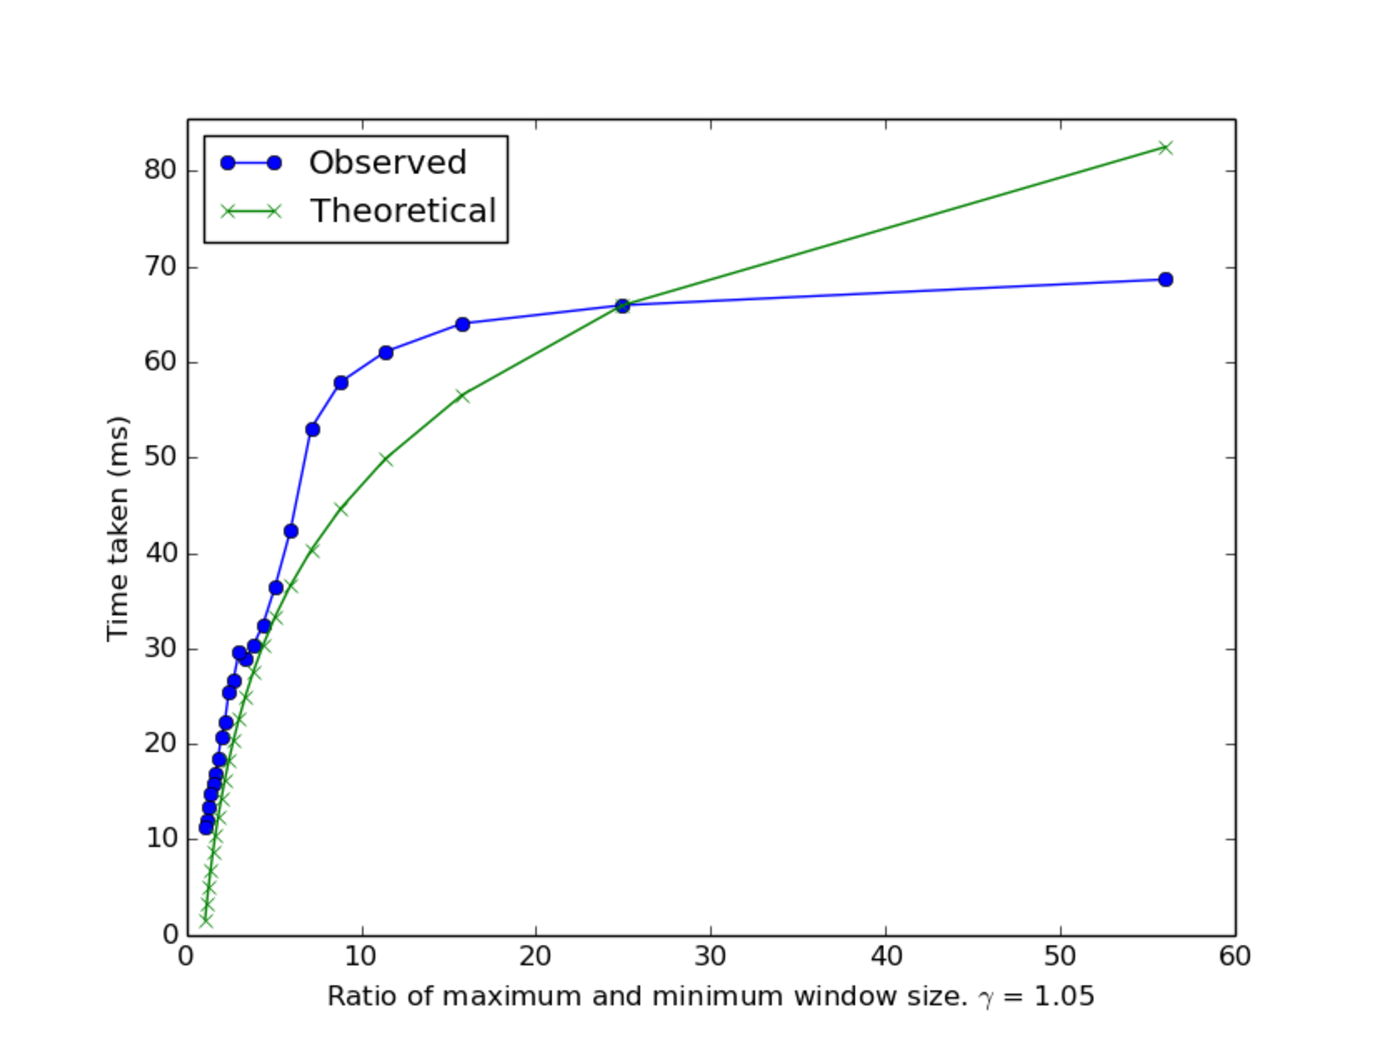
\includegraphics[width=\textwidth]{Appendices/figures1/winSize_vs_time}
    \caption{Comparison of ratio of maximum and minimum search window size with time taken taken for detection. It is clear from the shape of curve (blue) connecting the time taken for every search size that it varies logarithmically. The ideal curve (green) is just shown as a reference of a log curve and is not metrically accurate because we are trying to explain the theoretical complexity.}
    \label{one}
\end{figure}

\paragraph{}
The resolution of each source image captured by the camera that form the panorama is $1920 \times 2560$. But as mentioned before, because of the various aisle section depths and camera perspective the search rectangle size has to vary across the average size. The search size characterized by the ratio of maximum and minimum window size is started from $W_{min}=(480, 274)$, $W_{max}=(518, 296)$ and broadened till $W_{min}=(63, 35)$, $W_{max}=(980, 560)$. In every iteration, the gap between the minimum and maximum window size is reduced by a step size $s = 24$ pixels, $i.e$ the minimum height is increased by 12 pixels and maximum height is decreased by 12 pixels with their corresponding widths being aspect ratio adjusted. The final time of detection for a given search gap is found by averaging the detection time over 291 images having slightly varying target object size. Fig. $\ref{one}$ shows the various search size represented by the ratio of maximum and minimum window sizes plotted against the detection time(blue dots connected by a blue line). It can be seen from the shape of the curve that it approximates the logarithmic complexity. The green curve is the true log curve plotted with the ratio of maximum and minimum window size, $i.e. \ log_\gamma(\frac{W_{max}^i}{W_{min}^i})$. This experiment empirically verifies that the detection time scales logarithmically with the search size.

\paragraph{}
The second experiment is to empirically verify that the detection time varies \textit{inverse logarithmically} with the increase in the scale factor, which is the step size from the minimum to maximum window size of detection. The experiment was conducted with the constant minimum window size $W_{min}=(63, 35)$ and maximum window size $W_{max}=(980, 560)$. The scale factor, $\gamma$ is increased in steps of 0.02 starting from $\gamma = 1.01$. It can be seen from the plot in Fig. \ref{two} that the detection time decreases inverse logarithmically with the increase in scale factor as explained theoretically by Eqn. \ref{eq9}. The green curve in Fig. \ref{two} is the ideal curve that is plotted with the different scale factors and constant detection window size using the formula derived in Eqn. \ref{eq9}, $i.e. \ log_{\gamma_i}(\frac{W_{max}}{W_{min}})$.

\begin{figure}[h]
    \centering
    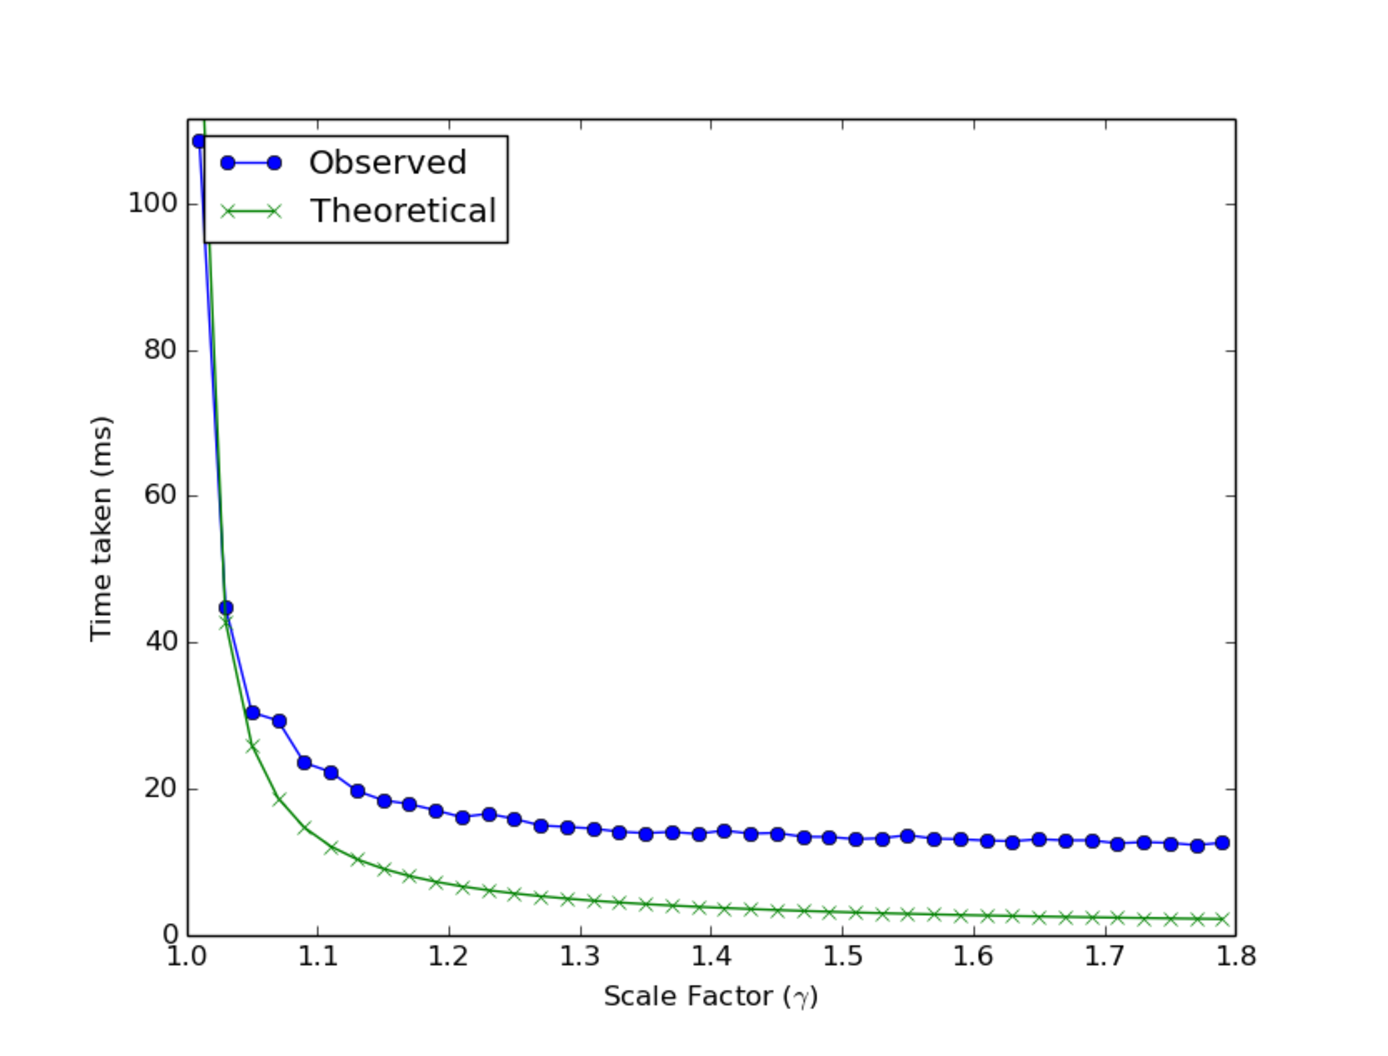
\includegraphics[width=\textwidth]{Appendices/figures1/gamma_vs_time}
    \caption{Comparison of scale factor with time taken taken for detection. It is clear from the shape of curve (blue) connecting the time taken for every scale factor that it varies \textit{inverse} logarithmically. The ideal curve (green) is just shown as a reference of a inverse log curve and is not metrically accurate because we are trying to explain the theoretical complexity.}
    \label{two}
\end{figure}
